\section{Task 8 at SemEval 2024}
\label{sec:task}

The 18th International Workshop on Semantic Evaluation (SemEval-2024) was a large event in NLP, offering various challenges that teams across the world could undertake.
Task 8 at SemEval-2024 \citep{wang2024semeval} centered around machine-generated text detection in a black-box setting (i.e., the generator models for the test set were not known while the competition was ongoing), in both monolingual and multilingual components.

This shared task spanned 3 subtasks: subtask A a binary classification task between generated and human texts, subtask B consisted in multi-class classification between multiple LLM generators, as well human texts, while subtask C was a boundary detection problem, where participants had to correctly pinpoint the boundary between a human and a machine-generated segment in each test.
During the active phase of SemEval-2024, which ended in February 2024, I undertook Task 8 jointly with Daniel Stuhlinger, a fellow student at the University of Tübingen.
The full report of our participation, carried out under the team name "TueCICL", can be viewed in \citet{stuhlinger-winkler-2024-tuecicl}.

As team TueCICL, we submitted results for two of the subtasks to the leaderboards, namely subtask A and subtask C, which were the two subtasks involving classification between solely human and machine-generated texts, whereas subtask B focused more on inter-generator differentiation.
For subtask A, consisting in binary classification over the whole texts, there were two phases development, one for shared task proper, and subsequent post-deadline experimenting in the context of this Master Thesis.
Due to the more pronounced research interest in subtask A, as well as to better present the higher volume of material associated with it, this section shall first discuss subtask C, then dive deeper into subtask A later in this Chapter.

\subsection{Human - LM Boundary detection}

Subtask C of the shared task addresses detection environments that are characterized by active adversarial agents performing the generation.
Specifically, detection technologies have been observed to be weak to techniques also found in authorship obfuscation \citep{macko2024authorship}, such as paraphrasing \citep{krishna2024paraphrasing} and noise-introduction \citep{wang2021adversarial}.
Change point detection, which is the titular requirement of subtask C, addresses another way in which the use of NLG technology might be obfuscated.
In the scenario targeted by the subtask, a human segment ranging from 0\% to 50\% of the text is concluded by a machine-generated component, making the text as a whole much harder to flag as a generation.

For all subtasks, the data is sourced from the M4 \citep{wang-etal-2024-m4} dataset.
Task organizers provided generations by GPT variants and the LLaMA series \citep{touvron2023llama}, but unfortunately not in high abundance: the training set contained around 5000 texts, and was accompanied by development set containing a little over 500 more.
Table \ref{fig:taskc_data} offers an overview of the data distribution across the sets.
Alongside the general scarcity of training and cross-validation data, one should also note that a relevant portion of the data is entirely machine-generated, meaning the change index is exactly 0.
Though this of course preserves the objective of being able to reliably detect fully generated texts, it does cut into the already low amount of true change examples available for training.

The evaluation metric by which the submitted solutions are measured is Mean Absolute Error (MAE), i.e. the average absolute difference in the predicted change-point index and the true value.
The baseline suggested by the organizers was based on Longformer \citep{beltagy2020longformerlongdocumenttransformer}, a fine-tuned RoBERTa checkpoint specialized in long texts.
This baseline achieved an impressive 3.5 MAE on the development set -- a tough standard -- and a (much lower) 21.54 MAE on the test set, though the latter was of course not known at development time.

\vspace{1cm}

\begin{table}[h]
    \centering
    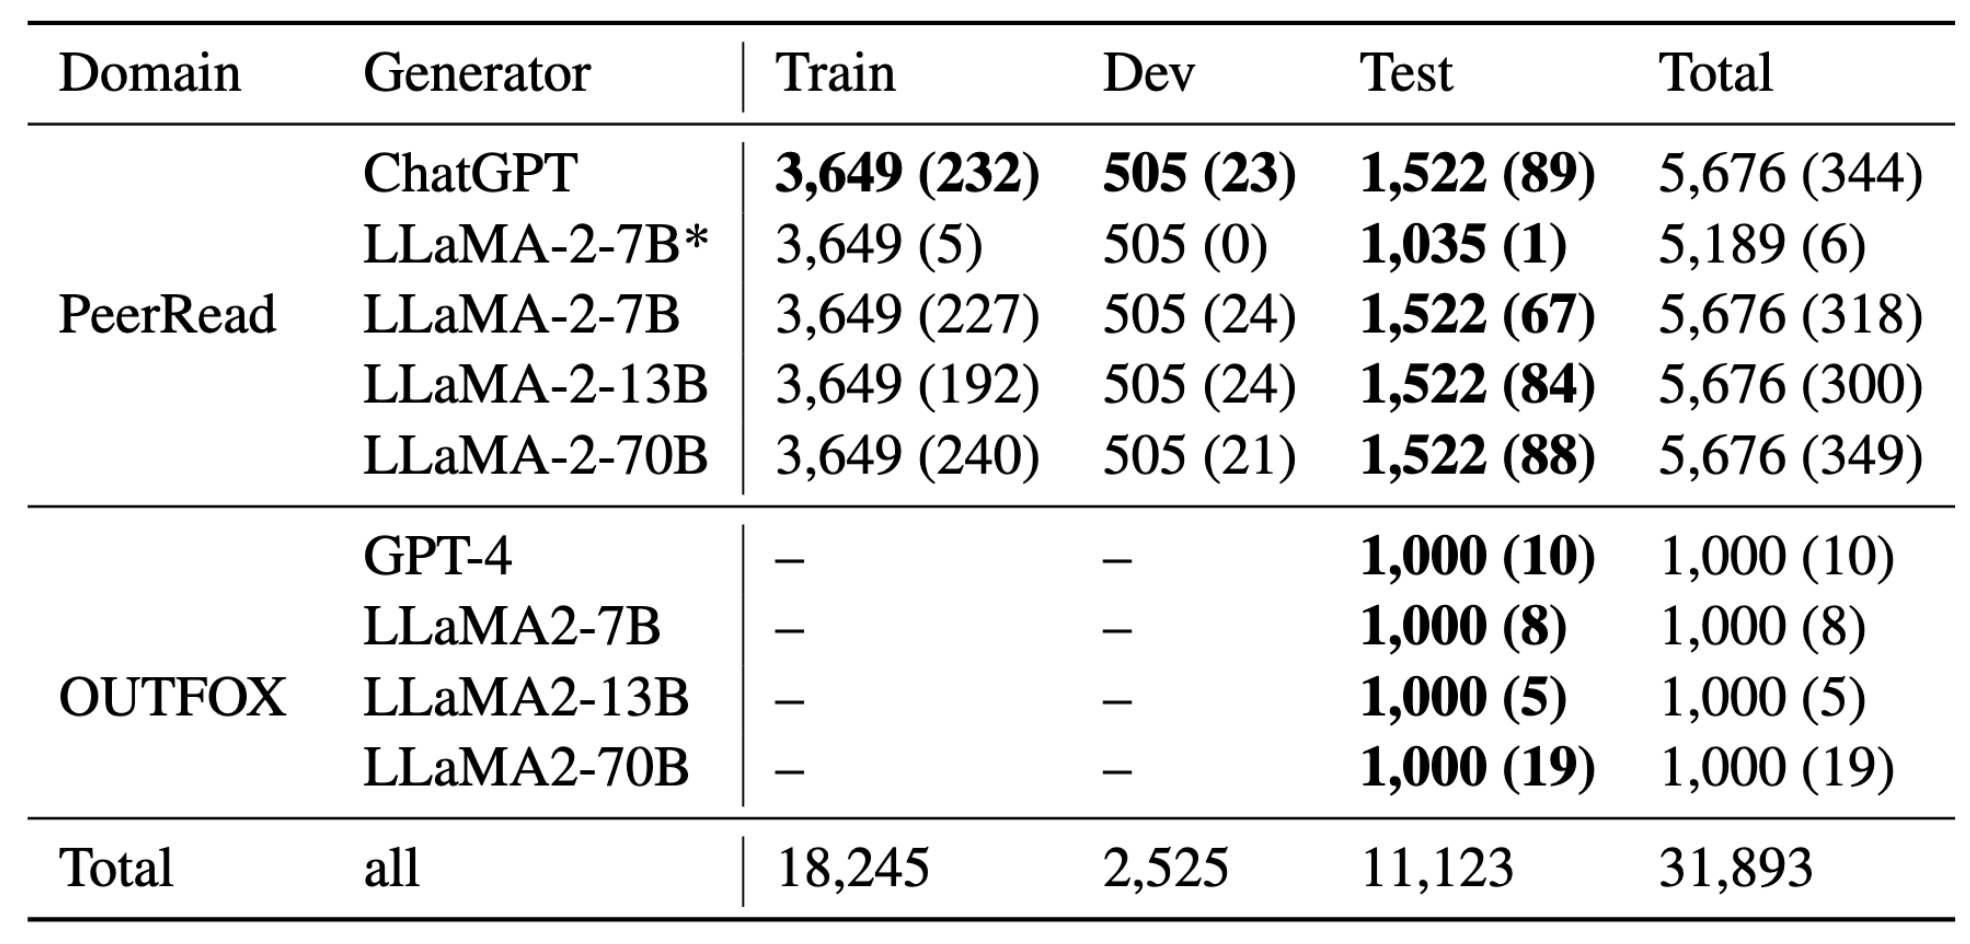
\includegraphics[width=0.7\textwidth]{assets/subtaskc-data.png}
    \caption{
        Dataset breakdown for subtask C from Task 8 at SemEval-2024.
        The number in “()” is the number of examples purely generated by LLMs, i.e., human and machine boundary index=0.
        LLaMA-2-7B* and LLaMA-2-7B used different prompts. Bold data is used in shared task training development, and test.
    }
    \label{fig:taskc_data}
\end{table}

Following the example set by the baseline, the solutions we devised did not attempt to predict the boundary change index directly -- instead, we performed binary classification at the token level, essentially asking whether any given token belongs to the human or the machine-generated segment.
In accordance with the general mission of producing solutions that could run on at least midrange home computers and laptops, large-scale transformer-based approaches, such as the one provided as the baseline, were discarded altogether.

Instead, we presented an ensemble model sourcing its input from two bidirectional long short-term memory, or LSTM \citep{hochreiter1997long}, models.
The first LSTM operated at the character level and did not include any elements of pertaining.
Preprocessing the input texts for this character-level model involved lowercasing, and mapping numerals and punctuation to a \verb|<NUM>| and a \verb|<PUNCT>| special token respectively.
Similarly, whitespace characters of any type (e.g. space, tab, newline) were also mapped to the special token \verb|<WS>|.
Classification then proceeds as outlined on the character level, and the first occurrence of the positive label (indicating that the token belongs to the machine segment) is taken as the boundary change index.
Naturally, the character-level index is traced back to the word-level position, as required by the task setting, where the position of the word in which the first positively classified character is located is taken as the final label.

The second LSTM relied on pretrained Word2Vec \citep{mikolov2013efficientestimationwordrepresentations} embeddings sourced from the Wiki2Vec project \citep{yamada2020wikipedia2vec}. Static embeddings have fallen out of favor lately due to the emergence of contextual embeddings derived from LLMs, but they offer the significant advantage of not requiring firing up a large language model at inference time, a property that made them well-suited for our objectives in subtask C.
While this LSTM performs word-level classification, as opposed to the character-level nature of the first model, many of the preprocessing steps are maintained.
Casting texts to lowercase letters is all the more relevant since the Word2Vec mapping is case sensitive, and also maintained mapping numerals, punctuation and white-space to special tokens.

At least on paper, employing pretrained Word2Vec embeddings introduces an important amount of information into the model that would not be possible to obtain solely based on the available training data.
However, for the character-level LSTM, there are no such mitigating factors.
From very early on, it was clear from intermediate results that the character-level LSTM struggled significantly, since it had no pretrained semantic context for the input letter sequences.
To address this excessive burden placed on the scarce training data to both inform on how human language works, as well as how to distinguish it from generations, we enrich the dataset provided for subtask C with that of subtask A.
While deep discussion of the latter is reserved for the later sections of this chapter, it should suffice to say that training data for subtask A contains over 100.000 records, providing ample linguistic material, albeit not targeted to the specific objective of subtask C.

Records imported from the training set for subtask A had the target label set to either 0 (for fully machine-generated texts), or the length of the tokenized text (for fully human texts).
Since this operation carries the inevitable side effect of drowning out the far fewer examples where a change occurs mid-text (which are available in subtask C's data only), all models are trained for 5 epochs on the enriched data, and then exclusively on the original task data.
Aside from the aforementioned optimizations, hyperparameter tuning over the characteristics of the models yielded that, for both LSTM's, a hidden size of 512 and 2 layers resulted in the highest validation performance.

After training the two base approaches, an ensemble model was also constructed combining the representations of the two LSTM's.
This consisted in a non-recurrent feed-forward network (FFN) whose inputs were the concatenated representations at the word level.
We applied this FFN head to the representations at each word-level token, outputting a binary label, the same way as the two LSTM's.
For the character-level model, this meant averaging the representation at every character for any given word, before passing the representation to the ensemble classifier, along with the Word2Vec-based model's embeddings.
Utilizing a simple FFN in this case was deemed to be the most efficient solution, since the interaction between the various elements of the sequence is already captured in the sub-models.
This is also similar to how token-level classification is performed with transformers, with a feed-forward classification head applied at each token.
The best-performing hidden size for this model was found to be 256.
Table \ref{tab:c_models} offers a summary of the models developed for subtask C.

\begin{table}[h]
    \centering
    \begin{tabular}{llll}
        \hline
        \textbf{Model}  & \textbf{Type}          & \textbf{Number of LSTM layers} & \textbf{Hidden size} \\
        \hline
        Character-level & Long short-term memory & 2                              & 512                  \\
        Word2vec        & Long short-term memory & 2                              & 512                  \\
        Joint model     & Feed-forward network   & -                              & 256                  \\
        \hline
        \vspace{0.1cm}
    \end{tabular}
    \caption{Summary of models for subtask C. \textbf{*} Number of layers. \textbf{**} Hidden size.}
    \label{tab:c_models}
\end{table}


\subsection{Generated text detection}
\label{subsec:subtask_a}

Subtask A of Task 8 tackles machine-generated text detection in the classical sense, in the way that was discussed in Chapter \ref{sec:approaches}.
It offered both a monolingual and a multilingual track, both with their respective leaderboards, but our team decided to only submit for the monolingual track.

As hinted at in the previous section, the training set provided for this subtask contained over 100.000 records, with 5000 more provided for validation, sourced from the M4 \citep{wang-etal-2024-m4} dataset.
Table \ref{table:adata} offers an overview of the data distribution across the three partitions.
All sets offer a balanced mix of generated and human texts, with the training set containing outputs from 4 different models: Davinci-003 (a GPT-3 variant), ChatGPT, Cohere \footnote{\url{https://cohere.com/}} and Dolly-v2 \citep{DatabricksBlog2023DollyV2}. The development set adds BLOOMz \citep{muennighoff2023crosslingualgeneralizationmultitaskfinetuning} to the collection, and the test set introduces GPT-4 on top.
The intent of the authors to enforce a black-box setting shines through in the way they built the partitions: the development set includes a model unknown to the train set, and the test set contains another model absent from the other splits.

\begin{table}[ht]
    \centering
    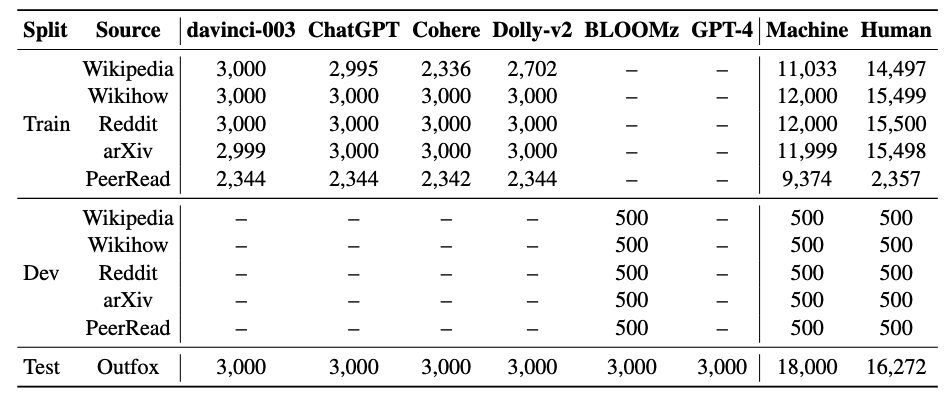
\includegraphics[width=0.8\textwidth]{assets/subtaska-data.png}
    \caption{Subtasks A: Monolingual Binary Classification. Data statistics over Train/Dev/Test splits.}
    \label{table:adata}
\end{table}


\subsection{Generated text detection: post-deadline additions}